%=======================================================
\section{Monitoring mit Skripten}
%=======================================================
Für die Überwachung von speziellen Anwendungen oder Arbeitsabläufen, reichen bestehende standardisierte Managementagenten häufig nicht aus. Die notwendigen Statusinformationen können über Standard- oder Herstellerspezifische \emph{SNMP MIB} nicht abgefragt werden. Um hier spezielle Anforderungen erfüllen zu können ist es möglich eigene Programme oder Skripte zur Überwachung einzubinden. Um ein möglichst praxisnahes und durchgängiges Beispiel liefern zu können, konfigurieren wir exemplarisch eine Festplattenüberwachung mit \emph{S.M.A.R.T}\abbrev{S.M.A.R.T.}{\markup{S}elf-\markup{M}onitoring, \markup{A}nalysis and \markup{R}eporting \markup{T}echnology}. Um die Abläufe zu verdeutlichen richten wir einen  Monitor ein, der den Zustand einer lokal installieren Festplatte überwacht.

Die Verwendung der eigenen Programme und Skripte kann auf unterschiedliche Art und Weise realisiert werden. Im ersten Teil wird beschrieben, wie der unter \emph{Unix/Linux} weit verbreitete \emph{Net-SNMP} Agent erweitert und in \emph{OpenNMS} genutzt werden kann. Das Monitoring des Festplattenstatus wird in Varianten durchgeführt und soll den Ablauf und die Notwendigen Konfigurationsschritte verdeutlichen.

\emph{Nagios}, als ein weit verbreitetes quelloffenes Monitoringsystem, stellt einen sehr großen Pool\footnote{Nagios Plugins unter \url{http://www.monitoringexchange.org}} von Überwachungsskripten und Programmen zur Verfügung. Diese Skripte können als \emph{Plugins} auf einem Server mit einem \emph{Nagios-Agenten}\footnote{Unter Linux/Unix \emph{NRPE}\abbrev{NRPE}{\markup{N}agios \markup{R}emote \markup{P}lugin \markup{E}xecutor} unter Windows \emph{NSClient++}} ausgeführt werden. In diesem Dokument wird beschrieben wie \emph{OpenNMS} die \emph{NRPE} Agenten in der Netzwerküberwachung nutzen kann. In \emph{OpenNMS} wird dazu ein spezieller \emph{NRPE Monitor} bereitgestellt. Er veranlasst das ausführen der \emph{Plugins} und stellt den Status entsprechend dar.

Da für die Verwaltung von \emph{Unix/Linux} basierten Systemen häufig das SSH-Protokoll\abbrev{SSH}{\markup{S}ecure \markup{Sh}ell} verwendet wird, kann auch dieses Protokoll für die Netzwerküberwachung verwendet werden. Es erlaubt neben der Bereitstellung eines entfernten Shellzugangs ebenfalls die Möglichkeit, Programme oder Skripte auf dem entfernten Server auszuführen. In \emph{OpenNMS} kann dazu der \emph{General Purpose Monitor} verwendet werden. Er erlaubt es Shellkommandos auszuführen und kann das Ergebnis des Kommandos in einem \emph{Service Status} auswerten.

Das \emph{HTTP}\abbrev{HTTP}{\markup{H}yper \markup{T}ext \markup{T}ransfer \markup{P}rotocol} ist eines der wichtigsten Protokolle im Internet. Es wird neben der Auslieferung von Internetseiten auch für entfernte Funktionsaufrufe (\emph{ReST}\abbrev{ReST}{\markup{Re}presentational \markup{S}tate \markup{T}ransfer} oder \emph{SOAP}\abbrev{SOAP}{\markup{S}imple \markup{O}bject \markup{A}ccess \markup{P}rotocol}) genutzt. Zusätzlich lässt sich \emph{HTTP} auch für Monitoring-Zwecke verwenden. Über \emph{HTTP} können sowohl Statusabfragen oder auch Leistungsdaten für das Monitoring bereitgestellt werden. Die Übertragung kann zudem über \emph{SSL}\abbrev{SSL}{\markup{S}ecure \markup{S}ocket \markup{L}ayer} verschlüsselt erfolgen. Zusätzlich sind Webserver nahezu auf jedem System sehr einfach einzurichten und sind im Netzwerk oft gut erreichbar. Im letzten Abschnitt wird gezeigt wie man einen \emph{Apache2-Server\footnote{Apache Project: \url{http://httpd.apache.org}}} in Verbindung mit \emph{CGI}\abbrev{CGI}{\markup{C}ommon \markup{G}ateway \markup{I}nterface} für das Monitoring in \emph{OpenNMS} einrichten kann. Der Fokus liegt hier auf dem Statusmonitoring. Auf eine \emph{HTTP-Datacollection\footnote{OpenNMS HTTP-Datacollection im OpenNMS Wiki}} zur Aufzeichnung von Leistungsdaten wird hier nicht eingegangen.

%=======================================================
\subsection{Einrichtung von S.M.A.R.T.}
%=======================================================
Um die Beispiele einrichten und nachvollziehen zu können muss voerst sicher gestellt werden, dass die \emph{S.M.A.R.T.-Tools} installiert und eingerichtet sind. Das folgende Beispiel wurde auf einem \emph{Ubuntu 9.10 Server} durchgeführt. Die \emph{S.M.A.R.T.-Tools} können mit dem folgenden Kommando installiert werden.

Für die Plattenüberwachung muss zusätzlich noch ein Prozess gestartet werden, der die entsprechenden Informationen von den Festplatten ausliest.

\begin{lstlisting}[numbers=none]
vi /etc/default/smartmontools
\end{lstlisting}

Zunächst muss erlaubt werden, dass der \emph{smartd} gestartet werden kann und welche Festplatten überwacht werden sollen. In unserem Beispiel werden die beiden Festplatten \emph{/dev/sda} und \emph{/dev/sdb} überwacht. Die Konfigurationsdatei sieht dann wie folgt aus:

\lstinputlisting[caption={Konfiguration der \emph{smartmontools}}
      \label{lst:smartmontools-config}]
  {configs/use-cases/script-extending-linux/smartmontools}

Der Dienst kann anschließend mit dem Kommando

\begin{lstlisting}[numbers=none]
service smartmontools start
\end{lstlisting}

gestartet werden. Um zu testen ob die Festplatteninformationen korrekt ausgelesen werden, kann das folgende Kommando den aktuellen Status liefern.

\begin{lstlisting}[numbers=none]
smartctl -H /dev/sdb
\end{lstlisting}

\lstinputlisting[caption={Ausgabe von \emph{smartctl}}
      \label{lst:smartctl-output}]
  {configs/use-cases/script-extending-linux/smartctl-output.txt}

Wenn die folgende Ausgabe wie oben gezeigt aussieht, dann können wir mit dem Einrichten der Überwachung fortfahren.

In den nächsten Abschnitten wird ein Monitoring mit den eben installierten smartmontools beschrieben. Wir beginnen zunächst mit der Variante über \emph{Net-SNMP}. Im Anschluss wird das gleiche Monitoring über \emph{NRPE}, über \emph{SSH} und auch über \emph{HTTP} mittels \emph{CGI} dargestellt.

\subsection{Net-SNMP als Agenten}
In \emph{Unix/Linux} Umgebungen kommt häufig \emph{Net-SNMP} als Agent zum Einsatz. Dieser stellt damit nicht nur den Zugriff für die in der \emph{Standard MIB-II} definierten Managementobjekte bereit, sondern erlaubt es zusätzlich eigene Skripte per \emph{SNMP} einzubinden. Diese Möglichkeit macht damit die Skripte und Programme nicht nur für \emph{OpenNMS} zugänglich, sondern können auch in jeder anderen \emph{SNMP-fähigen} Netzwerküberwachungsanwendung verwendet werden. In diesem Beispiel wird gezeigt wie ein Shellskript in \emph{Net-SNMP} eingebunden wird. Die Ausgabe des Skriptes wird mit dem \emph{OpenNMS} bereitgestellten \emph{SNMP-Monitor} überwacht und als \emph{Service-Status} dargestellt. In der folgenden Abbildung wird der Ablauf grob skizziert.

\begin{figure}[H]
	\centering
	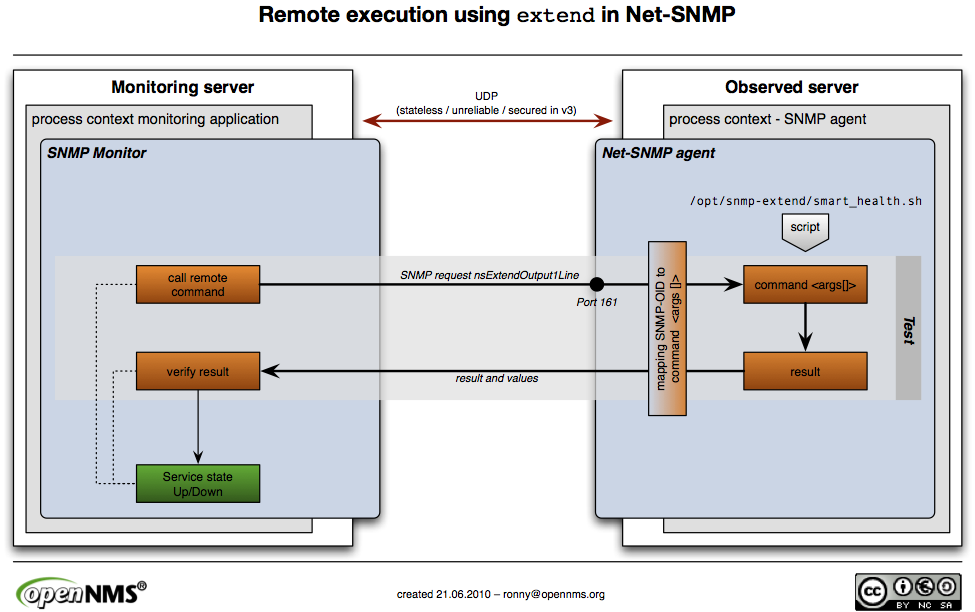
\includegraphics[width=1.0\textwidth]{images/use-cases/script-extending-linux/flow-netsnmp}
	\caption{Ablauf von Abfragen mit der Erweiterung des \emph{Net-SNMP} Agenten}
	\label{pic:flow-netsnmp}
\end{figure}

%=======================================================
\subsubsection{Grundeinrichtung von Net-SNMP}
%=======================================================
Damit die Einrichtung vollständig nachvollzogen werden kann, wird die Grundeinrichtung von \emph{Net-SNMP} kurz vorgestellt. In diesem Beispiel wird ebenfalls ein \emph{Ubuntu Server 9.10} verwendet. Die Installation der \emph{SNMP-Tools} und des \emph{Net-SNMP} Agenten erfolgt mit

\begin{lstlisting}[numbers=none]
aptitude install snmp snmpd
\end{lstlisting}

Nach erfolgreicher Installation kann der Agent mit dem Kommando

\begin{lstlisting}[numbers=none]
service snmpd start
\end{lstlisting}

gestartet werden. Ob der Agent funktioniert kann mit den SNMP-Tools getestet werden. Eine \emph{SNMP-Abfrage} über die installierte Kernelversion sieht dann wie folgt aus:

\begin{lstlisting}[numbers=none]
snmpget -v 2c -c public localhost .1.3.6.1.2.1.1.1.0
\end{lstlisting}

\begin{lstlisting}[numbers=none]
SNMPv2-MIB::sysDescr.0 = STRING: Linux marge 2.6.31-22-generic-pae \
#60-Ubuntu SMP Thu May 27 01:40:15 UTC 2010 i686
\end{lstlisting}

Mit dieser Abfrage wird die Systembeschreibung per \emph{SNMP} ausgelesen und liefert auf einem Unix/Linux-System die laufende Kernelversion.
Aus Sicherheitsgründen ist die Standardkonfiguration des \emph{SNMP-Agenten} sehr restriktiv konfiguriert. Der Agent lauscht nur auf der \emph{IP-Loopback} Schnittstelle und die Abfrage der kompletten MIB ist nicht gestattet. Damit eine entfernte Abfrage über das Netzwerk überhaupt möglich ist, müssen daher einige Anpassungen vorgenommen werden.

Im ersten Schritt setzen wir eine andere \emph{SNMP community}. Die \emph{Standard-Community} ist auf \emph{public} gesetzt. 

\textbf{\textit{Hinweis:}} Es macht Sinn eine unternehmensweite einheitliche \emph{Community} festzulegen, die nicht \emph{public} für den Lese- und \emph{privat} für den Schreibzugriff ist.

Zusätzlich erlauben wir den Zugriff auf den \emph{SNMP Agenten} nur der IP-Adresse des OpenNMS Servers. Die Angabe wird in \emph{CIDR}\abbrev{CIDR}{\markup{C}lassless \markup{I}nter \markup{D}omain \markup{R}outing}\footnote{Nach / wird die Anzahl der Bits für eine Bitmaske angegeben}-Schreibweise angegeben. Dazu bearbeiten wird die Konfigurationsdatei mit

\begin{lstlisting}[numbers=none]
vi /etc/snmp/snmpd.conf
\end{lstlisting}

\begin{lstlisting}
com2sec readonly  <opennms-server>/32     notpublic
.
group MyROGroup v2c        readonly
.
view all    included  .1                               80
.
access MyROGroup ""      any       noauth    exact  all    none   none
\end{lstlisting}

\emph{OpenNMS} genügt ein lesender Zugriff. Damit im Monitoring auf die komplette \emph{MIB} und nicht nur auf den Teilbaum system zugegriffen werden kann, ändern wir die \emph{com2sec\footnote{com2sec beschreibt eine Zuordnung einer Community auf ein Sicherheitsmodell}} von \emph{paranoid} auf \emph{readonly}. Anstelle von \emph{default} setzen wir die IP-Adresse des \emph{OpenNMS} Servers mit einer 32bit Maske ein. Die \emph{Community} ändern wir von public auf einen selbst definierten Wert, in diesem Beispiel einfach auf \emph{notpublic}.

Hinweis: Wenn Sie einen Standardzugriff für andere Anwendung mit der Community public benötigen, dann kann auch eine zweite Zeile mit einer weiteren Community eingefügt werden. Sie sollten dann allerdings den Sicherheitsmodus paranoid bei public stehen lassen. 

Der Zugriff auf den \emph{SNMP-Agenten} wird von einem entfernten Rechner allerdings noch nicht funktionieren, da der \emph{SNMP-Agent} standardmässig nur auf der \emph{IP-Loopback} Schnittstelle lauscht. Damit \emph{SNMP-Anfragen} von entfernten Rechnern beantwortet werden können, bearbeiten wir die folgende Datei mit

\begin{lstlisting}[numbers=none]
vi /etc/default/snmpd
\end{lstlisting}

und binden den Agenten auf alle IP-Adressen. Dazu ändern wird den Eintrag von \emph{127.0.0.1} auf \emph{0.0.0.0}. Bei oder bei \emph{multihomed\footnote{\emph{multihomed}bedeutet, dass Server mehr als eine Netzwerkschnittstelle besitzen}} Servern kann auch eine IP-Adresse auf einem speziellen Netzwerkadapter gewählt werden. Die entsprechende Zeile sollte dann wie folgt aussehen:

\begin{lstlisting}
# snmpd options (use syslog, close stdin/out/err).
SNMPDOPTS='-Lsd -Lf /dev/null -u snmp -I -smux -p /var/run/snmpd.pid \
0.0.0.0'
\end{lstlisting}

Nach einem Neustart des SNMP-Agenten mit

\begin{lstlisting}[numbers=none]
service snmpd restart
\end{lstlisting}

können SNMP-Anfragen von entfernten Rechnern durchgeführt werden. Die Einstellung kann mit dem Kommando

\begin{lstlisting}[numbers=none]
netstat -lnpu
\end{lstlisting}

überprüft werden. Die Ausgabe sollte dann wie folgt aussehen:

\begin{lstlisting}[numbers=none]
udp        0      0 0.0.0.0:161           0.0.0.0:*             17391/snmpd
\end{lstlisting}

Ein Test von einem entfernten Rechner kann mit dem Kommando

\begin{lstlisting}[numbers=none]
snmpwalk -v 2c -c notpublic <snmp-agent-host>
\end{lstlisting}

durchgeführt werden. Im Folgenden wird die komplette \emph{MIB}, mit allen entsprechenden Werten, auf der Konsole ausgegeben. Damit sind die Voraussetzungen geschaffen um mit der Einrichtung des Monitorings fortzufahren.

%=======================================================
\subsubsection{Ein Skript zur Ermittlung des SMART-Status}
%=======================================================
Nach erfolgreicher Installation der \emph{smartmontools} schreiben wir ein kleines Wrapper-Skript, welches uns das entsprechende Ergebnis auswertet und auf der Konsole ausgibt. Die Ausgabe werden wir später über \emph{SNMP} zugänglich machen. Das Skript sieht hier wie folgt aus:

\lstinputlisting[caption={Wrapper-Skript für \emph{smartctl}}
      \label{lst:wrapper-smartctl}]
  {configs/use-cases/script-extending-linux/check_smart_health.sh}
  
Hinweis: Es ist hilfreich sich die Skripte einheitlich an einer zentralen Stelle abzulegen. Die Pflege und Wartung wird damit wesentlich erleichert. 

Hier in diesem Beispiel werden die Skripte im Verzeichnis \emph{/opt/snmp-extend} gespeichert. Mit dem ersten Parameter geben wir an, von welcher Festplatte wir den Status prüfen möchten. Damit das Kommando ausgeführt werden kann, müssen die entsprechenden Rechte gesetzt werden:

\begin{lstlisting}[numbers=none]
chmod +x /opt/snmp-extend/check_smart_health.sh
\end{lstlisting}

Wir können nun das Skript testen und erhalten eine folgende Ausgabe, wenn wir die erste Festplatte prüfen:

\begin{lstlisting}[numbers=none]
cd /opt/snmp-extend
./smart_health /dev/sda
\end{lstlisting}

\begin{lstlisting}[numbers=none]
SMART overall-health self-assessment test result: PASSED
\end{lstlisting}

Da das Kommando \emph{smartctl} lediglich als Benutzer \emph{root} ausgeführt werden kann, der \emph{SNMP Agent} allerdings mit dem Benutzer \emph{snmp} gestartet wird, müssen wir uns hier entsprechende Rechte für den \emph{SNMP-Benutzer} zuweisen. Eine mögliche Lösung wäre es in der \emph{/etc/default/snmpd} den Parameter \emph{-u} von \emph{snmp} auf \emph{root} zu ändern. Das hätte dann allerdings zur Folge, dass alle Aktionen vom \emph{SNMP Agenten} unter \emph{root} Rechten ausgeführt werden. Wir gehen einen anderen Weg und verwenden hierzu sudo und erlauben lediglich das ausführen der Skripte unter \emph{/opt/snmp-extend} als Benutzer \emph{root}.

Wir bearbeiten mit dem Kommando \emph{visudo} die Datei \emph{/etc/sudoers} und fügen die folgende Zeile hinzu:

\begin{lstlisting}[numbers=none]
# Allow snmp daemon to execute extended commands as root
snmp    ALL=NOPASSWD: /opt/snmp-extend/*.sh
\end{lstlisting}

Damit ist sichergestellt, dass der Benutzer \emph{snmp} nur Dateien mit dem Suffix \emph{.sh} im Verzeichnis \emph{/opt/snmp-extend} mit \emph{sudo} starten kann. Für die Ausführung ist keine Kennworteingabe notwendig. Im nächsten Schritt erweitern wir \emph{Net-SNMP Agenten} mit den entsprechenden Skripten.

%=======================================================
\subsubsection{Erweiterung von Net-SNMP}
%=======================================================
Der Agent \emph{Net-SNMP} bietet uns selbst wiederum verschiedene Möglichkeiten an, damit ein Skript oder Programm über eine \emph{OID}\abbrev{OID}{\markup{O}bject \markup{Id}entifier} angesprochen werden kann. Wir verwenden die Anweisung \emph{extend} und bearbeiten dazu die Datei \emph{snmpd.conf}.

\begin{lstlisting}[numbers=none]
vi /etc/snmpd.conf
\end{lstlisting}

um sie um die folgenden Einträge zu erweitern. Da zwei Festplatten im Server vorhanden sind, wird das Skript entsprechend mit den beiden \emph{Blockdevices} als Parameter aufgerufen.

\lstinputlisting[caption={Erweiterung \emph{Net-SNMP} mit dem erstellten Wrapper-Skript für \emph{smartctl}}
      \label{lst:snmp-extend-config}]
  {configs/use-cases/script-extending-linux/snmp-extend.cfg}

Damit die Änderungen wirksam werden, muss der \emph{SNMP-Agent} mit

\begin{lstlisting}[numbers=none]
service snmpd restart
\end{lstlisting}

neu gestartet werden. Die entsprechenden Skripte können jetzt mit \emph{SNMP} abgerufen werden.

\textbf{\textit{Hinweis}}: Unter \emph{Debian} können benutzerdefinierte Einstellungen auch in der Datei \emph{/etc/snmp/snmpd.local.conf} gesetzt werden. Damit sind alle rechnerspezifischen Einträge in einer speraten Datei ausgelagert und Roll-Outs sowie Updates sind leichter administrierbar.

\begin{lstlisting}[numbers=none]
snmpwalk -v 2c -c notpublic <snmp-agent-host> nsExtendOutput1Line
\end{lstlisting}

\begin{lstlisting}[numbers=none]
NET-SNMP-EXTEND-MIB::nsExtendOutput1Line."smart_health_sda" = STRING: SMART \
overall-health self-assessment test result: PASSED

NET-SNMP-EXTEND-MIB::nsExtendOutput1Line."smart_health_sdb" = STRING: SMART \
overall-health self-assessment test result: PASSED
\end{lstlisting}

Das Skript wird ausgeführt und die Ausgabe unter den oben gezeigten OIDs per SNMP bereitgestellt. Um den entsprechenden SNMP-Monitor in OpenNMS einzurichten, benötigen wir die vollständige OID zu den entsprechenden Ausgaben. Diese lässt sich mit dem Kommando

\begin{lstlisting}[numbers=none]
snmpwalk -On -v 2c -c notpublic <snmp-agent-host> nsExtendOutput1Line
\end{lstlisting}

anzeigen. Die entsprechenden \emph{OIDs} sehen dann wie folgt aus:

\begin{lstlisting}[numbers=none]
.1.3.6.1.4.1.8072.1.3.2.3.1.1.16.115.109.97.114.116.95.104.101.97.108.116. \
104.95.115.100.97

.1.3.6.1.4.1.8072.1.3.2.3.1.1.16.115.109.97.114.116.95.104.101.97.108.116. \
104.95.115.100.98
\end{lstlisting}

Die \emph{OIDs} werden dabei wie folgt aufgebaut. Der erste Teil der \emph{SNMP-OID} adressiert alle eingebundenen Skripte.

\begin{lstlisting}[numbers=none]
.1.3.6.1.4.1.8072.1.3.2.3.1.1.16
\end{lstlisting}

der zweite Teil der \emph{SNMP-OID} wird der "Name" des Skriptes in \emph{Hex-Dezimal\footnote{JavaScript ASCII Bin-Hex-Dec Converter: \url{http://mediusrete.org/diversions/ascii-conv.html}}} Zahlen angegeben. s=115, m=109, a=97 usw. Aus \emph{smart\_health\_sda} wird dann 

\begin{lstlisting}[numbers=none]
115.109.97.114.116.95.104.101.97.108.116.104.95.115.100.97
\end{lstlisting}

Es können so Skripte als Net-SNMP Erweiterungen eindeutig adressiert werden. Das Bedeutet im Umkehrschluss, dass jeder Name in der Anweisung extend nur einmal verwendet werden kann und eindeutig sein muss.

%=======================================================
\subsubsection{Einrichtung SNMP-Monitor in OpenNMS}
%=======================================================
OpenNMS hat verschiedene Möglichkeiten Monitore bereitzustellen, welcher über die Methode \emph{Discovery} und dem \emph{Capsd\footnote{Capabilityscan Daemon - Dienst zur automatischen Erkennung von Monitoren und Protokollen}} sowie über \emph{Provisioning Groups\footnote{Provisioning Groups sind konkret definierte Netzwerkgeräte die im Monitoring bereitgestellt werden}} angelegt werden können. Wir verwenden \emph{Capsd}, um den Dienst auf allen Servern automatisch zu erkennen. In der Datei wird ein entsprechendes Protokoll wie folgt angelegt:

\begin{lstlisting}[numbers=none]
vi $OPENNMS_HOME/etc/capsd-configuration.xml
\end{lstlisting}

Das Protokoll wird in \emph{XML-Syntax}\abbrev{XML}{E\markup{x}tensible \markup{M}arkup \markup{L}anguage} wie folgt angelegt:

\lstinputlisting[caption={Konfiguration von \emph{capsd} zum automatischen erkennen des Service für \emph{sda} und \emph{sdb}}
      \label{lst:smart-capsd-snmp-config}]
  {configs/use-cases/script-extending-linux/smart-capsd-snmp-config.xml}

\textbf{\textit{Hinweis:}} Bitte fügen Sie eigene Monitore am Ende der Datei an und markieren Sie den Bereich wo eigene Monitore angelegt wurden. Bei einem Update wird es damit wesentlich einfacher die entsprechende Konfiguration zu überführen.

\textbf{\textit{Wichtig:}} In der Darstellung sind Zeilenumbrüche mit \ gekennzeichnet. In der Konfigurationsdatei von \emph{OpenNMS} sollten die entsprechenden Angaben in einer Zeile angegeben werden.

Auf allen Servern bei denen sich diese \emph{SNMP-OID} abfragen lässt bindet, \emph{OpenNMS} den Monitor auf die entsprechende IP-Schnittstelle des Knotens und überacht dessen Status automatisch. Im nächsten Schritt muss ein entsprechender Monitor eingerichtet werden, welcher den entsprechenden Status überprüft. Dazu wird die Konfigurationsdatei für den \emph{Pollerd\footnote{Pollerd testet ob der \temph{SMART} Status ok ist oder nicht.}} wie folgt bearbeitet:

\begin{lstlisting}[numbers=none]
vi $OPENNMS_HOME/etc/poller-configuration.xml
\end{lstlisting}

\lstinputlisting[caption={Konfiguration von \emph{pollerd} zum testen des Service für \emph{sda} und \emph{sdb}}
      \label{lst:smart-poller-snmp-config}]
  {configs/use-cases/script-extending-linux/smart-poller-snmp-config.xml}

Die beiden Monitore können im Bereich \emph{polling-package} "example1" angegeben werden. Es ist hier ebenfalls sinnvoll die eigenen Monitore in der Konfiguration zu markieren und am Ende anzufügen. Am Ende der Datei muss noch festgelegt werden von welchem Typ der Monitor ist. In unserem Fall sind beide vom Typ \emph{SnmpMonitor}.

Damit die Einstellungen übernommen werden, sollte zunächst die Konfiguration mit \emph{xmllint\footnote{Unter \emph{Ubuntu} kann \emph{xmllint} über das Kommando \emph{aptitude install libxml2-utils} installiert werden.}}

\begin{lstlisting}[numbers=none]
xmllint $OPENNMS_HOME/etc/capsd-configuration.xml
xmllint $OPENNMS_HOME/etc/poller-configuration.xml
\end{lstlisting}

getestet werden. Nach erfolgreichem Test muss OpenNMS mit dem Kommando

\begin{lstlisting}[numbers=none]
service opennms restart
\end{lstlisting}

neu gestartet werden. Mit einem \emph{Rescan} auf einem bestehendem Knoten\footnote{Als Knoten wird ein Server, Router oder anderes Netzwerkkgerät in \emph{OpenNMS} bezeichnet}. wird geprüft ob die entsprechenden Skripte erfolgreich aufgerufen werden können und anschließend von \emph{OpenNMS} überwacht.

\textbf{\textit{Wichtig:}} Beachten Sie die eingestellten \emph{Timeouts} im \emph{SNMP-Monitor}. Die Laufzeit der lokalen Skripte sollte diese \emph{Timeouts} nicht überschreiten. Der \emph{SNMP-Agent} verwendet intern einen \emph{Cache} und speichert im Standard die letzten Ergebnisse für 5 Sekunden. 

\textbf{\textit{Hinweis:}} Den \emph{Cache} des \emph{SNMP-Agenten} kann man für jedes Skript seperat konfigurieren. Mit dem Kommando

\begin{lstlisting}[numbers=none]
snmpset -v2c -c notpublic <snmp-agent-host> 'NET-SNMP-EXTEND-MIB::nsExtendCacheTime."smart_temp_sda"' i 15
\end{lstlisting}

\begin{lstlisting}[numbers=none]
NET-SNMP-EXTEND-MIB::nsExtendCacheTime."smart_temp_sda" = INTEGER: 15
\end{lstlisting}

wird die Zeit für den \emph{Cache} für den Eintrag \emph{smart\_temp\_sda} auf 15 Sekunden gesetzt. 

Mittels dieser Methode lassen sich ebenfalls Leistungsdaten mit dem \emph{Collectd\footnote{Collectd wird der Collection Daemon genannt der Leistungsdaten für Trendanalyse in \emph{RRD-Dateien} aufzeichnet.}} zur Langzeitarchivierung und Trendanalyse durchführen. Die entsprechende Konfigurationen sind im \emph{OpenNMS Wiki\footnote{Beschreibung Datacollection \url{http://www.opennms.org/index.php/Data\_Collection\_Configuration_How-To}}} dokumentiert. Im nächsten Abschnitt wird die Überwachung mit dem Nagios Agenten NRPE dargestellt.

%=======================================================
\subsection{NRPE als Agent}
%=======================================================
\emph{Nagios} ist ein sehr weit verbreitetes Netzwerkmonitoring-Tool. Für \emph{Nagios} selbst sind zahlreiche \emph{Plugins\footnote{Eine Plugin Datenbank wird unter \url{http://www.monitoringexchange.org} angeboten}} vorhanden. Um die entsprechenden \emph{Plugins} auf entfernten Systemen auszuführen, stellt \emph{Nagios} einen eigenen Agenten \emph{NRPE} bereit. \emph{Nagios} kann über ein IP-Netzwerk ein \emph{Plugin} entfernt ausführen und bekommt das entsprechende Ergebnis übermittelt. Mit \emph{OpenNMS} können ebenfalls \emph{Nagios Plugins} über den \emph{NRPE-Agent} abgefragt werden. Im folgenden wird gezeigt wie ein \emph{Plugin} von \emph{Nagios} zur Ermittlung des \emph{SMART-Status} mit \emph{OpenNMS} und dem \emph{NRPE-Monitor} getestet werden können.

\begin{figure}[H]
	\centering
	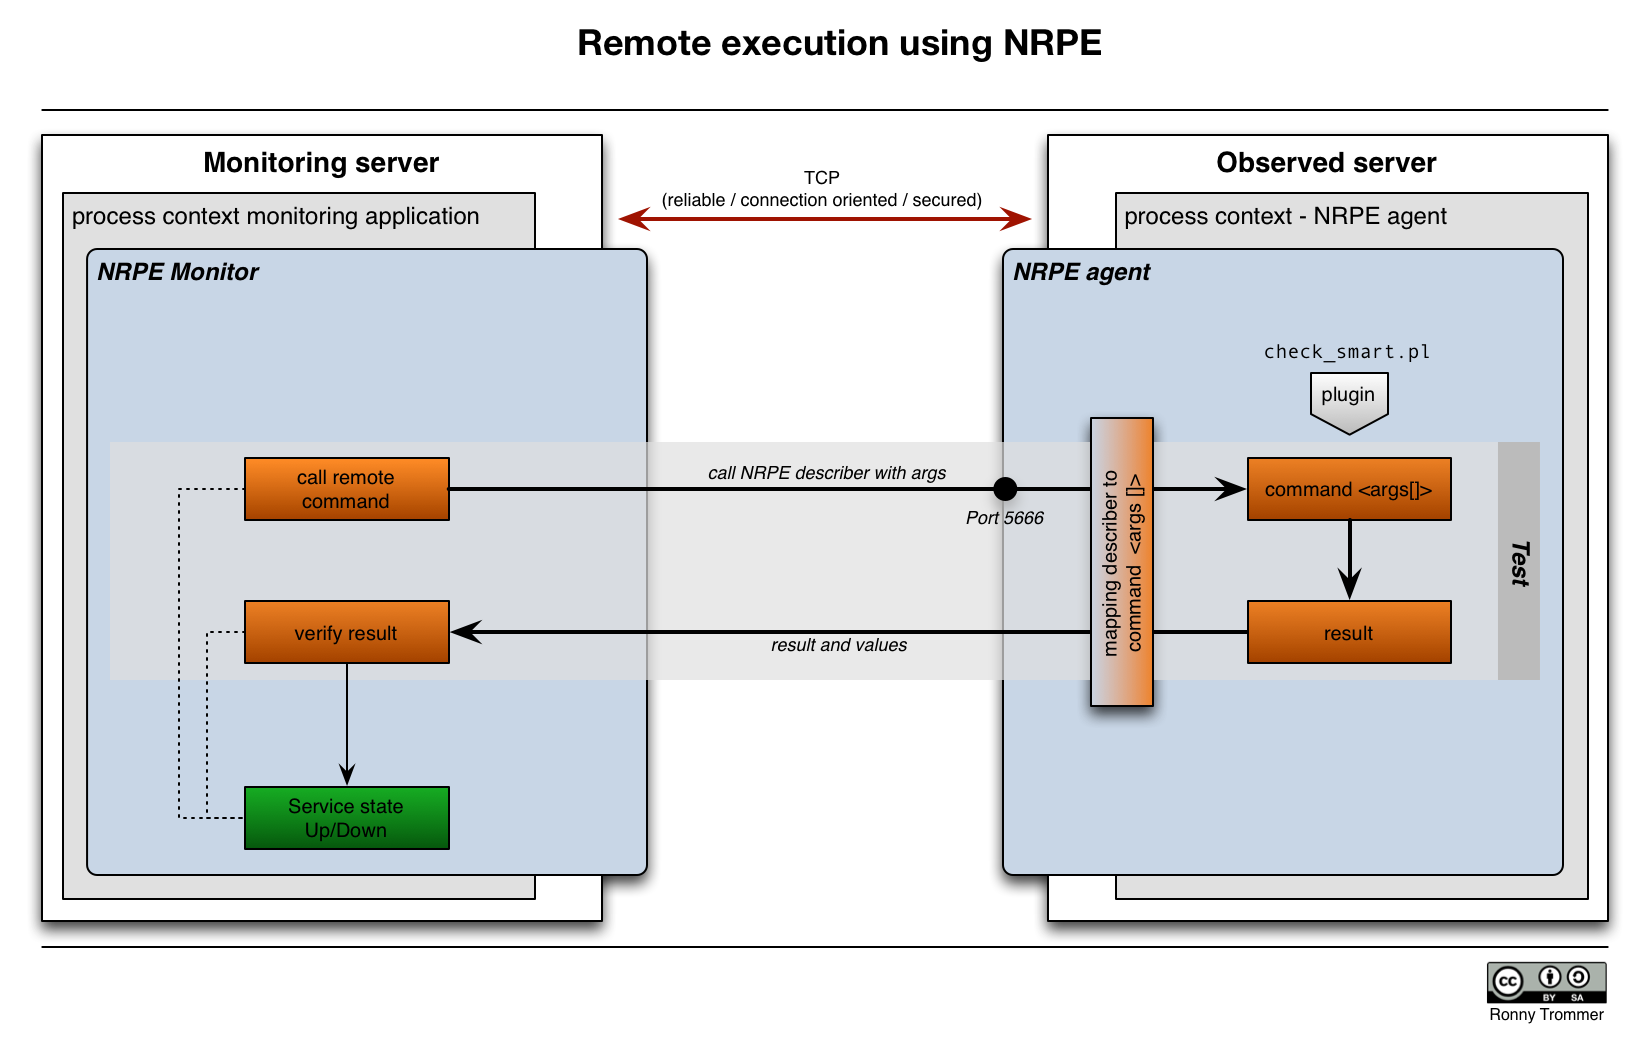
\includegraphics[width=1.0\textwidth]{images/use-cases/script-extending-linux/flow-nrpe}
	\caption{Ablauf von Abfragen über den \emph{NRPE} Agenten}
	\label{pic:flow-nrpe}
\end{figure}

%=======================================================
\subsubsection{Grundeinrichtung von NRPE}
%=======================================================
Bevor wir mit der Einrichtung des \emph{Plugins} beginnen, wird gezeigt wie der \emph{NRPE} eingerichtet werden muss. Die Installation des \emph{NRPE-Agenten} auf einem \emph{Ubuntu 9.10 Server} kann mit dem Kommando

\begin{lstlisting}[numbers=none]
aptitude install nagios-nrpe-server
\end{lstlisting}

erfolgen. Aus Sicherheitsgründen ist der \emph{NRPE-Agent} sehr restriktiv konfiguriert. Es werden lediglich Anfragen von \emph{127.0.0.1} erlaubt. Damit der \emph{OpenNMS Server} auf die \emph{Plugins} zugreifen kann, wird die IP-Adresse in \emph{allowed\_hosts} eingetragen.

\begin{lstlisting}[numbers=none]
vi /etc/nagios/nrpe.cfg
\end{lstlisting}

\begin{lstlisting}[numbers=none]
allowed_hosts=127.0.0.1,<opennms-host>
\end{lstlisting}

Im nächsten Schritt muss ein entsprechendes \emph{Plugin} eingerichtet und über \emph{NRPE} zugänglich gemacht werden. Für den \emph{NRPE-Agenten} können zusätzliche Startparameter in der Datei \emph{nagios-nrpe-server} in \emph{/etc/default} bearbeitet werden. Um beispielsweise \emph{SSL} zu deaktivieren, kann die Option \emph{--nossl} angegeben werden:

\begin{lstlisting}[numbers=none]
vi /etc/default/nagios-nrpe-server
\end{lstlisting}

\begin{lstlisting}[numbers=none]
DAEMON_OPTS="--no-ssl"
\end{lstlisting}

%=======================================================
\subsubsection{Ein Nagios-Plugin für den SMART Status}
%=======================================================
Für diese Beispiel verwenden wir das Plugin \emph{check\_smart\footnote{\url{http://www.monitoringexchange.org/inventory/Check-Plugins/Hardware/Storage/Check-SMART-status}}}. Damit das \emph{Plugin} ausgeführt werden kann, ist ein \emph{Perl Interpreter} notwendig. Zusätzlich muss die \emph{Nagios} eigene \emph{Perl} Bibliothek \emph{utils.pm\footnote{Die Bibliothek \emph{utils.pm} wird mit den \emph{Nagios Plugins} ausgeliefert}} installiert sein. Das \emph{Plugin} kopieren wir in das Verzeichnis \emph{/usr/lib/nagios/plugins}. Die \emph{Plugins} müssen zunächst ausführbar gemacht werden:

\begin{lstlisting}[numbers=none]
chmod +x /usr/lib/nagios/plugins/check_smart.pl
\end{lstlisting}

Die Funktion des Plugins kann mit dem Kommando

\begin{lstlisting}[numbers=none]
check_smart.pl -d /dev/sda -i scsi
\end{lstlisting}

getestet werden. Die Ausgabe sollt wie unten gezeigt aussehen.

\begin{lstlisting}[numbers=none]
OK: no SMART errors detected
\end{lstlisting}

Das Plugin muss anschließend im \emph{NRPE-Agenten} eingetragen werden. Dazu wird die Datei \emph{nrpe\_local.cfg} wie folgt erweitert:

\begin{lstlisting}[numbers=none]
vi /etc/nagios/nrpe_local.cfg
\end{lstlisting}

\begin{lstlisting}[numbers=none]
command[check_smart_sda]=/usr/lib/nagios/plugins/check_smart.pl -d /dev/sda - scsi

command[check_smart_sdb]=/usr/lib/nagios/plugins/check_smart.pl -d /dev/sdb - scsi
\end{lstlisting}

Damit das neu eingerichtete Plugin genutzt werden kann, muss der NRPE-Agent mit dem Kommando 

\begin{lstlisting}[numbers=none]
service nagios-nrpe-server restart
\end{lstlisting}

neu gestartet werden. Mit einem entsprechendem \emph{check\_nrpe\footnote{NRPE: \url{http://www.nagios-wiki.de/nagios/howtos/nrpe}}} Plugin kann der Dienst jetzt wie folgt getestet werden:

\begin{lstlisting}[numbers=none]
check_nrpe -H <nrpe-host> -c check_smart_sda
\end{lstlisting}

\begin{lstlisting}[numbers=none]
OK: no SMART errors detected
\end{lstlisting}

Bei der Auswertung des Ergebnisses ist allerdings nicht die Ausgabe sondern der \emph{exit code} relevant. \emph{Nagios} kennt nicht nur \emph{UP} oder \emph{DOWN}. Die exit codes sind dabei wie folgt zugeordnet:

\pagebreak

\begin{longtable}{|p{3.5cm}|p{5cm}|p{5cm}|}
  % Kopf auf erste Seite
  \hline
    \rowcolor{light_gray}[5.8pt]
 	 Exit code	&	NRPE-Status & OpenNMS-Status\\
	 \hline
	 \endfirsthead
	 %Kopf auf weiteren Seiten
	 \hline \multicolumn{3}{|c|}{(Fortsetzung)}\\
	 \hline
	 \rowcolor{light_gray}[5.8pt]
 	 Exit code	&	NRPE-Status & OpenNMS-Status\\
	 \hline
	 \endhead
	 \hline
	 \multicolumn{3}{|c|}{(Tabelle wird auf der nächsten Seite fortgesetzt)}
  \endfoot
  \hline
	\caption{Zuweisung von NRPE zu OpenNMS Status codes}
  \endlastfoot
	\hline
  	0    &    Ok    &    Up \\
  	\hline
  	1    &    Warning    &    Down \\
  	\hline
  	2    &    Critical    &    Down \\
  	\hline
  	3    &    Unknown    &    Down \\
  	\hline
  	4    &    Dependent    &    Down
   \label{tbl:nrep-opennms-status}
\end{longtable}

Mit den oben gezeigten Einstellungen kann nun der \emph{OpenNMS Monitor} eingerichtet werden. Da auch der \emph{NRPE-Agent} unter einem restriktivem Benutzer läuft, muss für Kommandos die \emph{root-Rechte} benötigen ein entsprechender \emph{sudo-Eintrag} vorgenommen werden.

\begin{lstlisting}[numbers=none]
visudo
\end{lstlisting}

\begin{lstlisting}[numbers=none]
nagios  ALL=NOPASSWD: /usr/lib/nagios/plugins/check*
\end{lstlisting}

Mit diesem Eintrag wird dem Benutzer \emph{nagios} erlaubt alle Plugins die mit \emph{check} beginnen über \emph{sudo} auszuführen.

%=======================================================
\subsubsection{Einrichtung NRPE-Monitor in OpenNMS}
%=======================================================
Damit \emph{OpenNMS} automatisch erkennen kann, wo das \emph{SMART-Status} \emph{Plugin} installiert ist, wird in der \emph{Capsd} wie folgt eingerichtet.

\begin{lstlisting}[numbers=none]
vi $OPENNMS_HOME/etc/capsd-configuration.xml
\end{lstlisting}

\lstinputlisting[caption={Konfiguration von \emph{capsd} zum automatischen erkennen des Service für \emph{sda} und \emph{sdb} mit dem \emph{NRPE-Plugin}}
      \label{lst:smart-capsd-nrpe-config}]
  {configs/use-cases/script-extending-linux/smart-capsd-nrpe-config.xml}

\textbf{\textit{Hinweis:}} Der \emph{NRPE-Agent} verschlüsselt die Übertragung standardmässig mit \emph{SSL}. Werden sowohl verschlüsselte als auch unverschlüsselte \emph{NRPE-Agenten} eingesetzt, ist es sinnvoll die entsprechenden Monitore mit \emph{NRPE} oder \emph{NRPES} als Protokollname zu kennzeichnen. Bei unverschlüsselten \emph{NRPE-Agenten} muss zusätzlich die Eigenschaft

\begin{lstlisting}[numbers=none]
<property key="usessl" value="false" />
\end{lstlisting}

gesetzt werden. Fehlt die Angabe wird von einer \emph{SSL}-verschlüsselten Kommunikation ausgegangen.

Um ein \emph{NRPE Plugin} vom \emph{OpenNMS Server} testen zu können, kann über die Kommandozeile das \emph{CheckNrpe Plugin} direkt ausgeführt werden. Leider kann über die Kommandozeile \emph{CheckNrpe} nur \emph{NRPE-Agenten} ansprechen die kein \emph{SSL} verwenden. Für \emph{Debugging-Zwecke} sollte das allerdings ausreichen. Es kann somit geprüft werden ob die Kommunikation von OpenNMS zum NRPE-Agenten funktioniert und die entspechenden Plugins richtig eingerichtet sind. Achten Sie auf die Versionsnummer des Java-Archives!

\begin{lstlisting}[numbers=none]
cd $OPENNMS_HOME/lib
java -cp opennms-services-1.8.0.jar org.opennms.netmgt.poller.nrpe.CheckNrpe -t 1 -H <nrpe-host> -c check_smart_sda
\end{lstlisting}

Damit die beiden Plugins überwacht werden muss noch ein entsprechender Monitor eingerichtet werden. Dazu wird die Konfiguration für den Pollerd wie folgt bearbeitet:

\begin{lstlisting}[numbers=none]
vi $OPENNMS_HOME/etc/poller-configuration.xml
\end{lstlisting}

\lstinputlisting[caption={Konfiguration von \emph{pollerd} um den Service Status über das \emph{NRPE-Plugin} zu testen}
      \label{lst:smart-poller-nrpe-config}]
  {configs/use-cases/script-extending-linux/smart-poller-nrpe-config.xml}

Nach einem Neustart von OpenNMS mit dem Kommando

\begin{lstlisting}[numbers=none]
service opennms restart
\end{lstlisting}

werden die entsprechenden \emph{Plugins} überwacht.

%=======================================================
\subsection{SSH als Agent}
%=======================================================
Viele \emph{Linux} oder \emph{Unix-Server} werden über das Netzwerk mit  \emph{SSH} administriert. Mit \emph{SSH} können Programme über eine verschlüsselte Netzwerkverbindung ausgeführt werden. Neben der reinen Verwaltung kann \emph{SSH} auch für Monitoringaufgaben verwendet werden. In diesem Beispiel wird gezeigt wie mit \emph{OpenNMS} und einem \emph{General Purpose Monitor} der \emph{SMART-Festplattenstatus} überwacht werden kann. Zunächst muss allerdings sicher gestellt werden, dass der \emph{OpenNMS Server} Kommandos ohne Kennworteingabe auf dem entfernten Server per \emph{SSH} ausführen kann. Im Anschluss wird ein entsprechends Skript erzeugt und das Monitoring in \emph{OpenNMS} eingerichtet. Die Vorgehensweise ist dem \emph{Nagios-Plugin} \emph{check\_by\_ssh} sehr ähnlich.

\begin{figure}[H]
	\centering
	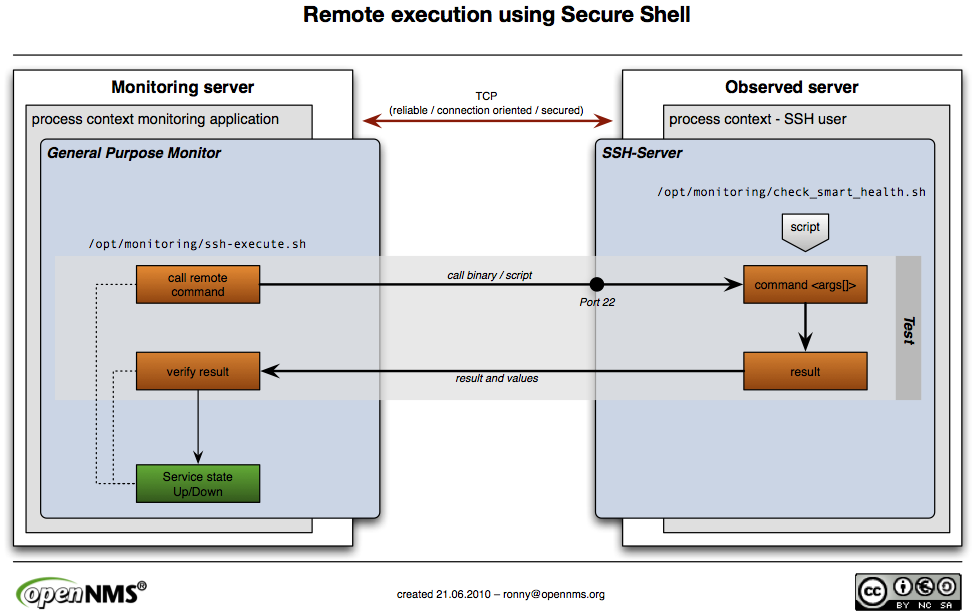
\includegraphics[width=1.0\textwidth]{images/use-cases/script-extending-linux/flow-ssh}
	\caption{Ablauf von Abfragen über \emph{SSH}}
	\label{pic:flow-ssh}
\end{figure}

%=======================================================
\subsubsection{Grundeinrichtung von SSH}
%=======================================================
Zur Ausführung von Kommandos über SSH ist eine Authentifizierung notwendig. Mit SSH kann eine Authentifizierung mittels Private- und Public Key und starker Verschlüsselung realisiert werden. Damit kein direkter root-Zugang besteht, wird auf dem entfernten Rechner ein Benutzer angelegt. Im gezeigten Beispiel ist auf dem lokalen sowie entfernten Server Ubuntu 9.10 installiert. Wir legen einen Benutzer monitoring an, der für diese Aufgaben entsprechend verwendet werden soll.

\begin{lstlisting}[numbers=none]
adduser monitoring
\end{lstlisting}

Für den Benutzer wird ein sicheres Kennwort eingerichtet. Zusätzlich erlauben wir dem Benutzer monitoring, das Ausführen der check-Skripte mit root-Rechten.

\begin{lstlisting}[numbers=none]
visudo
\end{lstlisting}

\begin{lstlisting}[numbers=none]
monitoring  ALL=NOPASSWD: /opt/monitoring/check*
\end{lstlisting}

Die entsprechenden Skripte zur Überwachung werden in einem zentralen Verzeichnis \emph{/opt/monitoring} gespeichert und von dort ausgeführt. Im nächsten Schritt wird ein privater und öffentlicher Schlüssel auf dem \emph{OpenNMS Server} generiert.

\begin{lstlisting}[numbers=none]
cd ~
ssh-keygen -t dsa
\end{lstlisting}

\begin{lstlisting}
Generating public/private dsa key pair.
Enter file in which to save the key (/root/.ssh/id_dsa):
Enter passphrase (empty for no passphrase): 
Enter same passphrase again: 
Your identification has been saved in id_dsa.
Your public key has been saved in ida_dsa.pub.
\end{lstlisting}

Das Schlüsselpaar bestehend aus privatem und öffentlichem Schlüssel und werden im Homeverzeichnis \emph{/root} gespeichert.

\textbf{\textit{Wichtig:}} Es darf keine \emph{Passphrase} eingegeben werden. Lediglich das Schlüsselpaar wird zur Authentifzierung verwendet.

Im Anschluss wird der öffentliche Schlüssel auf den entfernten Rechner kopiert. Der öffentliche Schlüssel muss auf dem entfernten Server im Verzeichnis \emph{Home-Verzeichnis} unter dem Verzeichnis \emph{.ssh} gespeichert werden. Wir befinden uns auf dem \emph{OpenNMS Server} und melden uns auf dem entfernten Rechner an. Als nächstes erstellen wir die entsprechenden Verzeichnisse und kopieren den öffentlichen Schlüssel auf den Server. Im Anschluss werden die Dateirechte entsprechend gesetzt.

\begin{lstlisting}[numbers=none]
# 1. .ssh Verzeichnis auf dem entfernten Server anlegen
ssh monitoring@<entfernter-server>
mkdir .ssh
exit
\end{lstlisting}

\begin{lstlisting}[numbers=none]
# 2. OpenNMS Server Verzeichnis /root
scp .ssh/id_dsa.pub monitoring@<entfernter-server>:/home/monitoring

ssh monitoring@<entfernter-server>
\end{lstlisting}

\begin{lstlisting}[numbers=none]
# 3. Public key fuer die Authentikation anlegen und Rechte setzen
cat id_dsa.pub >> .ssh/authorized_keys2
chmod 400 .ssh/authorized_keys2
chmod 500 .ssh
rm id_dsa.pub
exit
\end{lstlisting}

Nun kann eine Shell-Sitzung ohne Authentifizierung, von root auf den Benutzer monitoring auf dem entfernten Server geöffnet, werden. Um die Ausführung zu testen kann man sich nun vom OpenNMS Server das Verzeichnis /var/log auf dem entfernten Server anzeigen lassen:

\begin{lstlisting}[numbers=none]
ssh monitoring@<entfernter-server> ls /var/log
\end{lstlisting}

%=======================================================
\subsubsection{Ein Skript zur entfernten Ausführung}
%=======================================================
Um die Ergebnisse der Kommandos für den \emph{OpenNMS Monitor} aufzubereiten wird ein \emph{Wrapper-Skript} auf dem \emph{OpenNMS Server} erstellt welches die entsprechenden Ausgaben für den Monitor aufbereitet. Die Skripte sollten zentral in einem Verzeichnis gespeichert werden. In dem gezeigten Beispiel werden alle Skripte in \emph{/opt/monitoring} gespeichert. Wir verwenden das gleiche Skript \emph{check\_smart\_health.sh} wie bei der \emph{Net-SNMP} Variante.

\lstinputlisting[caption={Wrapper Skript für remote auszuführende \emph{SSH} Kommandos}
      \label{lst:ssh-execute}]
  {configs/use-cases/script-extending-linux/ssh-execute.sh}
  
Um zu testen ob das Kommando über \emph{SSH} ausgeführt wird, kann der folgende Aufruf verwendet werden:

\begin{lstlisting}[numbers=none]
ssh monitoring@<entfernter-server> /usr/bin/sudo "/opt/monitoring/check_smart_health.sh /dev/sda"
\end{lstlisting}

Alle entfernten Kommandos werden durch das Skript \emph{ssh-execute.sh} gestartet. Dem Skript wird zusätzlich noch ein Parameter für das zu testende \emph{Blockdevice} übergeben. \emph{Capsd} und \emph{Pollerd} übergeben automatisch die gerade zu prüfende IP-Adresse als 4. Parameter. Die IP-Adresse wird später von \emph{OpenNMS} dynamisch für die \emph{SSH-Verbindung} zum Test verwendet. Im nächsten Schritt wird der entsprechende Monitor eingerichtet.

%=======================================================
\subsubsection{Einrichtung General Purpose Monitor in OpenNMS}
%=======================================================
Damit \emph{OpenNMS} automatisch erkennt auf welchem Server \emph{SMART} mit den entsprechenden Überwachungsskripten installiert ist, richten zunächst ein Protokoll für den \emph{Capsd} ein. 

\lstinputlisting[caption={Konfiguration von \emph{capsd} zum automatischen erkennen des Service für \emph{sda} und \emph{sdb} mit \emph{SSH}}
      \label{lst:smart-capsd-ssh-config}]
  {configs/use-cases/script-extending-linux/smart-capsd-ssh-config.xml}

Im nächsten Schritt wird ein Monitor im \emph{Pollerd} eingerichtet. Hier wird über einen regulären Ausdruck geprüft ob tatsächlich der Status \emph{OK} ist und entsprechend in \emph{OpenNMS} gesetzt.

\lstinputlisting[caption={Konfiguration von \emph{pollerd} zum testen des Service für \emph{sda} und \emph{sdb} mit \emph{SSH}}
      \label{lst:smart-poller-ssh-config}]
  {configs/use-cases/script-extending-linux/smart-poller-ssh-config.xml}

Nach einem Neustart von \emph{OpenNMS} mit dem Kommando

\begin{lstlisting}[numbers=none]
service opennms restart
\end{lstlisting}

wird der Status des \emph{SMART-Status} überwacht. Auf jedem Server auf dem das Skript vorhanden und remote ausführbar ist, wird automatisch erkannt und in \emph{OpenNMS} automatisch überwacht.

\textbf{\textit{Wichtig:}} Die verschlüsselte Kommunikation über \emph{TCP} sowie das Ausführen externer Programme erzeugt zusätzlich schwergewichtige Prozesse mittels \emph{fork()}. Wenn Skalierbarkeit sehr stark im Vordergrund steht, ist die Variante über \emph{SNMP} zu bevorzugen.

\textbf{\textit{Hinweis:}} Man kann auch vor einem Test das Skript per \emph{scp} auf den Zielserver kopieren, ausführen und wieder entfernen. Damit kann ein zentrales Skript-Repository realisiert werden. Die Skalierbarkeit auf Seiten von \emph{OpenNMS} wird dann allerdings weiter reduziert, da ein einzelner Test weitaus mehr Ressourcen beansprucht.

%=======================================================
\subsection{Webserver als Agenten}
%=======================================================
Fast auf jedem Netzwerkgerät sind mittlerweile \emph{Webserver} zur Konfiguration und Kontrolle von Statusinformationen vorhanden. Zusätzlich ist das \emph{HTTP-Protokoll\footnote{HTTP Hyper Text Transfer Protokoll, man könnte es schon fast als Transportprotokoll des Internets nennen.}} eines der wichtigsten Protokolle in Internet- und großen Netzwerkumgebungen. Die Durchlässigkeit von \emph{HTTP(S)} über \emph{Firewall-Systeme} oder \emph{Proxies} ist sehr hoch. Damit kann sich dieses Protokoll ebenfalls sehr gut zur Überwachung über weit verteilte Standorte eignen.

Für die Überwachung verwenden wir den \emph{OpenNMS} integrierten \emph{HTTP-Monitor}. Dieser Monitor kann zum Einen \emph{Webserver} prüfen ob \emph{Web-Seiten} korrekt ausgeliefert und zum Anderen über reguläre Ausdrücke den Inhalt prüfen. In diesem Beispiel werden wir eine einfache \emph{HTTP-Seite} einrichten die uns den Status des \emph{smartctl} ausgibt. Den Status  testen wir dann anschließen mit dem \emph{HTTP-Monitor}. In dem gezeigten Anwendungsfall wird \emph{CGI\footnote{Common Gateway Interface URL:\url{http://httpd.apache.org/docs/2.0/howto/cgi.html}}} und ein \emph{Bash-Skript} verwendet. Es ist fast überall direkt verwendbar und hat sehr wenig weitere Abhängigkeiten.

\begin{figure}[H]
	\centering
	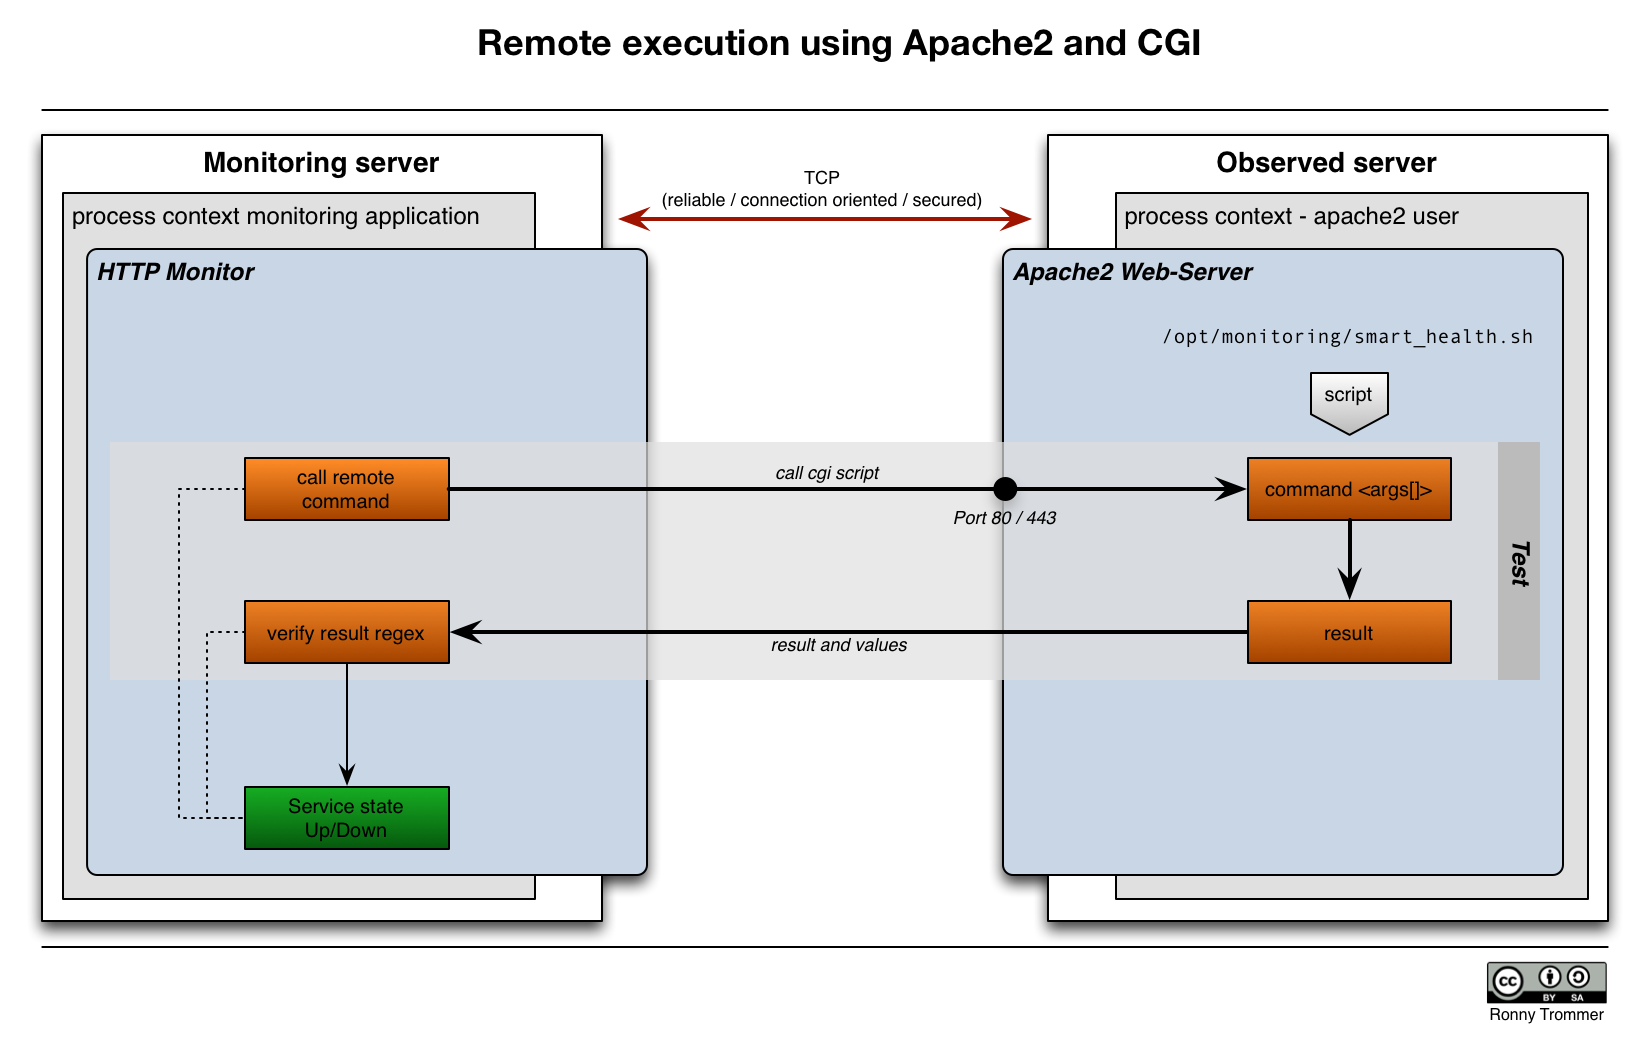
\includegraphics[width=1.0\textwidth]{images/use-cases/script-extending-linux/flow-cgi}
	\caption{Ablauf von Abfragen über \emph{CGI}}
	\label{pic:flow-cgi}
\end{figure}

\textbf{\textit{Hinweis:}} Es können natürlich analog \emph{PHP}, \emph{Perl} oder \emph{Python} als Sprache zum generieren der \emph{Web-Seite} verwendet werden.

Die hier gezeigte Konfiguration ist exemplarisch auf einem \emph{Ubuntu 9.10 Server} eingerichtet worden. Die Installation von \emph{apache2} wird mit dem folgenden Kommando durchgeführt.

\begin{lstlisting}[numbers=none]
aptitude install apache2
\end{lstlisting}

%=======================================================
\subsubsection{Einrichtung Apache2 mit CGI}
%=======================================================
Um die Ausführung von Kommandos über \emph{CGI} zu ermöglichen, erlauben wir das Ausführen von Skripten zum Monitoring mit der folgenden Konfiguration.

\begin{lstlisting}[numbers=none]
vi /etc/apache2/sites-available/default
\end{lstlisting}

durchgeführt. Wir fügen einen weiteren Skriptpfad an und schränken die Nutzung auf IP-Ebene auf den \emph{OpenNMS Server} ein.

\lstinputlisting[caption={Konfiguration von \emph{apache2} um \emph{CGI} Skripte auszuführen}
      \label{lst:apache2-cgi-config}]
  {configs/use-cases/script-extending-linux/apache2.cfg}

Der \emph{Webserver} benötigt für die Ausführung des Programms \emph{smartctl} \emph{root-Rechte}. Der \emph{Webserver} erhält daher die notwendigen Rechte um \emph{smartctl} mit \emph{sudo} aufrufen zu können. In dem Verzeichnis \emph{/opt/monitoring} erstellen wir ein Skript mit der Bezeichnung \emph{check\_smart\_health.sh}. 

\textbf{\textit{Wichtig:}} Um die Ausführung der Skripte einzuschränken muss anstelle von <ip-opennms> eine entsprechende Adresse oder Adressbereich angegeben werden. Es gibt zur Zeit keine Möglichkeit im \emph{HTTP-Monitor} eine Authentifizierung anzugeben. Der Zugang ist nur auf Basis von IP-Adressen oder Adressbereichen möglich.

Die Ausgabe des Skriptes wird über \emph{HTTP} zugänglich gemacht. Die Rechte werden mit dem Kommando

\begin{lstlisting}[numbers=none]
visudo
\end{lstlisting}

wie folgt eingerichtet:

\begin{lstlisting}[numbers=none]
www-data        ALL=NOPASSWD: /usr/sbin/smartctl
\end{lstlisting}

Als Parameter wird die entsprechend zu testende Festplatte mit übergeben. Wir benutzen für CGI das \emph{check\_smart\_health.sh}, wie wir es schon für \emph{SNMP}, \emph{NRPE} und \emph{SSH} verwendet haben.

Das Skript wird anschliessend mit dem Kommando

\begin{lstlisting}[numbers=none]
chmod +x check_smart_health.sh
\end{lstlisting}

ausführbar gemacht. Die Ausführung des Skriptes testen wir in einem Browser über die URL\abbrev{URL}{\markup{U}niform \markup{R}esource \markup{L}ocator}

\begin{lstlisting}[numbers=none]
http://<entfernter-server>/cgi-mon/check_smart_health.sh?/dev/sda
\end{lstlisting}

Die Ausgabe sollte dann wie folgt aussehen:

\begin{figure}[H]
	\centering
	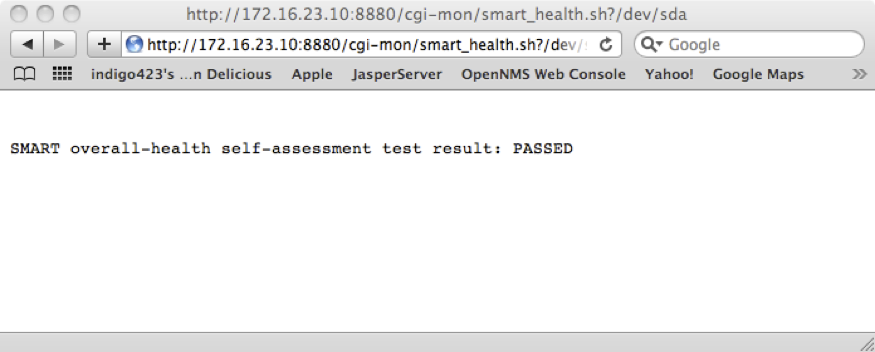
\includegraphics[width=1.0\textwidth]{images/use-cases/script-extending-linux/result-apache2-cgi}
	\caption{Ablauf von Abfragen über \emph{apache2} mit \emph{CGI}}
	\label{pic:flow-cgi}
\end{figure}

Auf diese Ausgabe kann nun ein \emph{HTTP-Monitor} eingerichtet werden. Wir nutzen dazu die Möglichkeit die Ausgabe mit einem regulärem Ausdruck zu prüfen.

%=======================================================
\subsubsection{Einrichtung HTTP-Monitor in OpenNMS}
%=======================================================
In diesem Beispiel wird \emph{Capsd} verwendet um die entsprechende Verfügbarkeit für das Monitoring automatisiert bereitzustellen. Der Monitor wird wie folgt angelegt:

\begin{lstlisting}[numbers=none]
vi $OPENNMS_HOME/etc/capsd-configuration.xml
\end{lstlisting}

\lstinputlisting[caption={Automatisches erkennen des \emph{CGI-Skriptes} für den \emph{S.M.A.R.T.} Festplattentest}
      \label{lst:lst:smart-capsd-cgi-config}]
  {configs/use-cases/script-extending-linux/smart-capsd-cgi-config.xml}

Um die entsprechende Ausgabe zu testen werden zwei HTTP-Monitore für den Pollerd in der Konfiguratonsdatei angelegt.

\begin{lstlisting}[numbers=none]
vi $OPENNMS_HOME/etc/poller-configuration.xml
\end{lstlisting}

\lstinputlisting[caption={Ausführen des Tests über das \emph{CGI-Skript} mit \emph{pollerd}}
      \label{lst:smart-poller-cgi-config}]
  {configs/use-cases/script-extending-linux/smart-poller-cgi-config.xml}
  
Nach einem Neustart von OpenNMS mit 

\begin{lstlisting}[numbers=none]
service opennms restart
\end{lstlisting}

wird das entsprechende Skript aufgerufen und die Ausgabe getestet. Die Ausführung lässt sich ebenfalls über \emph{HTTPS} verschlüsseln. Für den \emph{Capsd} muss dann lediglich ein \emph{HttpsPlugin} und im \emph{pollerd} ein \emph{HttpsMonitor} verwendet werden.

%=======================================================
\subsection{Fazit}
%=======================================================
Wie man sehen kann, sind die Möglichkeiten eigene Programme oder Skripte auszuführen sehr vielfältig. Die Entscheidung welche besser oder schlechter sind lässt sich pauschal nicht beantworten. Die Anforderungen an die Netzwerkinfrastruktur und entsprechende Sicherheitsrichtlinien sind sehr unterschiedlich. Aus diesem Grund werden hier eine Vor- und Nachteile der entpsrechenden Methoden beleuchtet. Die Anwendung lässt sich im Übrigen auch auf andere Netzwerk-Monitoring Anwendungen wie \emph{Nagios} oder \emph{Icinga} übertragen.

Im folgenden werden auf verschiedene Aspekte der Sicherheit, Wartbarkeit und Skalierbarkeit eingegangen.

\begin{longtable}{|p{3.5cm}|p{3.5cm}|p{3.5cm}|p{3.5cm}|}
  % Kopf auf erste Seite
  \hline
    \rowcolor{light_gray}[5.8pt]
 	 Agent    &    Wartbarkeit    &    Skalierbarkeit       &    Sicherheit \\
	 \hline
	 \endfirsthead
	 %Kopf auf weiteren Seiten
	 \hline \multicolumn{4}{|c|}{(Fortsetzung)}\\
	 \hline
	 \rowcolor{light_gray}[5.8pt]
 	 Agent    &    Wartbarkeit    &    Skalierbarkeit       &    Sicherheit \\
	 \hline
	 \endhead
	 \hline
	 \multicolumn{4}{|c|}{(Tabelle wird auf der nächsten Seite fortgesetzt)}
  \endfoot
  \hline
	\caption{Entscheidungshilfe für das Skript-Monitoring}
  \endlastfoot
	\hline
  	SNMP    &    -    &    ++    &    v1, v2c, v3 ++ \\
  	\hline
  	NRPE    &    -    &    +    &    + \\
  	\hline
  	SSH     &    +    &    -    &    + \\
  	\hline
  	HTTP    &    -    &    +    &    +
   \label{tbl:summary-implementation}
\end{longtable}

Bei \emph{SNMP}, \emph{NRPE} und \emph{HTTP} liegen auszuführende Skripte lokal auf jedem zu überwachendem Server. Die dezentrale Ablage muss mit entsprechenden Standards für ein Roll-Out in großen Umgebungen besonders berücksichtigt werden.

Bei \emph{SSH} besteht zusätzlich die Möglichkeit per \emph{scp} Skripte auf den Servern zu verteilen. Das kann ein Roll-Out erleichtern.

\emph{SNMP} bietet die höchste Skalierbarkeit. Durch das schlanke und verbindungslose Protokoll \emph{UDP}\abbrev{UDP}{\markup{U}ser \markup{D}atagram \markup{P}rotocol}, werden sehr wenig Ressourcen beansprucht. Auf dem \emph{OpenNMS Server} selbst können bei \emph{SNMP}, \emph{NRPE} und \emph{HTTP} die Monitor als leichtgewichtige \emph{Java-Threads} ausgeführt werden. 
Bei \emph{SSH} und dem \emph{General Purpose Monitor} werden für jeden Test mit \emph{fork()} ein Systemprozess erzeugt, was sich mit höherem Ressourcenverbrauch auf dem \emph{OpenNMS Server} bermerkbar macht. Zusätzlich werden bei Protokollen die auf \emph{TCP}\abbrev{TCP}{\markup{T}ransmission \markup{C}ontrol \markup{P}rotocol} basieren, eine verbindungsorientierte und bestätigte Kommunikation verwendet, die mehr Ressourcen verwendet. Bei \emph{SSH} kommt als zusätzlicher Aufwand noch die Verschlüsselung hinzu. In Umgebungen die durch \emph{Firewalls} abgesichert sind, lassen sich jedoch häufig \emph{TCP-basierende} Protokolle einfacher einsetzen.

Bei \emph{SNMP} (nur Version 3) kann eine Authentifizierung und Verschlüsselung verwendet werden. Bei \emph{NRPE}, \emph{SSH} und \emph{HTTP} ist lediglich eine Authentifizierung auf IP-Ebene Möglich. Jeder der \emph{root-Zugriff} auf den \emph{OpenNMS Server} hat kann die entsprechenden Kommandos oder \emph{Plugins} auf dem entfernten Server ausführen.
